%----------------------------------------------------------------------------------------
%	Metropolia Thesis LaTeX Template
%----------------------------------------------------------------------------------------
% License:
% This work is licensed under the Creative Commons Attribution 4.0 International License. To view a copy of this license, visit http://creativecommons.org/licenses/by/4.0/.
%
% Authors:
% Panu Leppäniemi, Patrik Luoto and Patrick Ausderau
%
% Credits:
% Panu Leppäniemi: abstract, def, cleaning,...
% Patrik Luoto: title page, abstract in Finnish, abbreviation, math,...
% Patrick Ausderau: initial version, style, table of content, bibliography, figure, appendix, table, source code listing...
%
% Please:
% If you find mistakes, improve this template and alike, please contribute by sharing your improvements and/or send us your feedback there: https://github.com/panunu/metropolia-thesis-latex
% And of course, if you improve it, add yourself as an author.
%
% Compiler:
% Use XeLaTeX as a compiler.

%----------------------------------------------------------------------------------------
%    ToDo
%----------------------------------------------------------------------------------------
% % % TÄRKEÄT
% % Translate "listing" in finnish (when inserting source code in the text)
% % Joku ifdef-tyyppinen vipu kieliversiolle (otsikot ja placeholdertekstit)
%    % Vaihtoehtona tietty erilliset filet suomelle ja enkulle, mutta
%    % tämä heikentää päivitettävyyttä (pitää aina muistaa korjata kahteen paikkaan).
%    % PA: I put CAPS comments where to switch depending on the language
% % Lisensointi (otsikkoon tekijä ja avoin lisenssi (esim. CC-BY, pohjan laatija
%   mainittava kommenttirivillä tjsp. [pohja ei ylitä teoskynnystä mutta kiva mainita].
%   PA: done
% % Projektin siirto Githubiin (siinä on issueträkkäys sun muut kivasti kunnossa) Vai?
%   %PA: done
% % Odotetaan 29.11.2013 asti äikänmaikkojen ja viestinnän mahdollisia kommentteja.
%   %done?
% %Reduce the vertical spacing for appendix in table of content
%   %done
%
% % % Vähemmän tärkeät
  % PNG:iden tilalle vektorigraffaa, jos vain löytyy kohtuuvaivalla

 
%----------------------------------------------------------------------------------------
%	THESIS
%----------------------------------------------------------------------------------------

\author{Uyiosa Imarhiagbe, Zoltán Gere, Albert Offei}
\title{Path follower(TM)}

\date{\today}
\def\metropoliadegree {Bachelor of Engineering}
\def\metropoliadegreeprogramme {Information Technology}
\def\metropoliaspecialisation {Smart Systems / Devices}
\def\metropoliainstructors {
Keijo Länsikunnas, Senior Lecturer\newline
Joseph Hotchkiss, Project Engineer}
\def\metropoliakeywords {Devices, Smart Systems, Embedded systems, Electronics}

%----------------------------------------------------------------------------------------
%	GLOBAL STYLES
%----------------------------------------------------------------------------------------

\documentclass[11pt,a4paper,oneside,article]{memoir}
%\usepackage[utf8]{inputenc}
%\usepackage[ansinew]{inputenc}
%\usepackage[T1]{fontenc}
%\usepackage[finnish]{babel} %IN ENGLISH, you can comment out or change this depending on your language
\usepackage[american]{babel} %IN ENGLISH, you can comment out or change this depending on your language
\usepackage{amsmath}
\usepackage{amsfonts}
\usepackage{amssymb}
\usepackage{fontspec}
\usepackage{tocloft}
%\usepackage{lipsum}
\usepackage{titlesec}
\usepackage[hyphens]{url}
\usepackage{mathtools}
\usepackage{wallpaper}
\usepackage{eso-pic}
\usepackage{datetime}
%\usepackage{lastpage} %other trick ;)
\usepackage{url}
\usepackage[amssymb]{SIunits}



\renewcommand{\dateseparator}{.}
%condition for adding or not space in TOC
\usepackage{etoolbox}
%for compact list
\usepackage{enumitem}
%for block comment
\usepackage{verbatim}
%for "easier" references
\usepackage{varioref}
%forcing single line spacing in bibliography
\DisemulatePackage{setspace}
\usepackage{setspace}
%including figure (image)
\usepackage{graphicx}
%change the numbering for figure
\usepackage{chngcntr}
%strike trough
\usepackage{ulem}
%euro symbol
\usepackage{eurosym}
%try to count
\usepackage{totcount}
%insert source code
\usepackage{listings}
\usepackage{caption}
\usepackage{color}
%force the width of a table instead of column
\usepackage{tabularx}

%NORMAL TEXT
%all text, title, etc. in the same font: Arial
%\setmainfont{Arial}
\setmainfont[
BoldFont=arialbd.ttf,
ItalicFont=ariali.ttf,
BoldItalicFont=arialbi.ttf
]{arial.ttf}
%line space
\linespread{1.5}
%\doublespacing
%margin
\usepackage[top=2.5cm, bottom=3cm, left=4cm, right=2cm, nofoot]{geometry}
\setlength{\parindent}{0pt} %first line of paragraph not indented
\setlength{\parskip}{16.5pt} %one empty line to separate paragraph
%list with small line space separation
\tightlists

%IMAGE - FIGURE
%the figures should be placed in the "illustration" folder
\graphicspath{{illustration/}}
%figure number without chapter (1.1, 1.2, 2.1) to (1, 2, 3)
\counterwithout{figure}{chapter}
%border around images
\setlength\fboxsep{0pt}
\setlength\fboxrule{0.5pt}
%caption font size
\captionnamefont{\small}
\captiontitlefont{\small}
%space after figure caption (and other float elements)
\setlength{\belowcaptionskip}{-7pt}

%TABLE
\counterwithout{table}{chapter}

%SOURCE CODE
%YOU NEED TO TRANSLATE THE CAPTION "Listing" in Finnish. 
%IN ENGLISH Nothing to do
\definecolor{darkgray}{rgb}{.4,.4,.4}
\definecolor{purple}{rgb}{0.65, 0.12, 0.82}
\lstset{
extendedchars=true,
captionpos=b,
caption=\footnotesize,
basicstyle=\singlespacing\ttfamily,%\small\fontfamily{"Courier"}\selectfont,
keywordstyle=\color{blue}\bfseries,
commentstyle=\color{purple}\itshape,
identifierstyle=\color{black},
stringstyle=\color{red},
showstringspaces=false,
showspaces=false,
numbers=left,
numberstyle=\footnotesize,
numbersep=9pt,
breaklines=true,
tabsize=2,
showtabs=false,
xleftmargin=1cm
}
%\counterwithout{lstlisting}{chapter}
%moved after begin document, otherwise does not compile

%TOC
%change toc title
%COMMENT OUT FOR ENGLISH
%\addto{\captionsfinnish}{\renewcommand*{\contentsname}{Sisällys}}
\renewcommand*{\contentsname}{Table of contents}
%remove dots
\renewcommand*{\cftdotsep}{\cftnodots}
%chapter title and page number not in bold
\renewcommand{\cftchapterfont}{}
\renewcommand{\cftchapterpagefont}{}
%sub section in toc
\setcounter{tocdepth}{2}
%subsection numbered
\setcounter{secnumdepth}{2}
\renewcommand{\tocheadstart}{\vspace*{-15pt}}
\renewcommand{\printtoctitle}[1]{\fontsize{13pt}{13pt}\bfseries #1}
\renewcommand{\aftertoctitle}{\vspace*{-22pt}\afterchaptertitle}
%spacing afer a chapter in toc
\preto\section{%
  \ifnum\value{section}=0\addtocontents{toc}{\vskip11pt}\fi
}
%spacing afer a section in toc
\renewcommand{\cftsectionaftersnumb}{\vspace*{-3pt}}
%spacing afer a subsection in toc
\renewcommand{\cftsubsectionaftersnumb}{\vspace*{-1pt}}
%appendix in toc with "Appendix " + num
\renewcommand*{\cftappendixname}{Appendix\space}

%TITLES
%chapter title
\titleformat{\chapter}
{\fontsize{13pt}{13pt}\bfseries\linespread{1}}
{\thechapter}{.5cm}{}
\titlespacing*{\chapter}{0pt}{.32cm}{9pt}
\titleformat{\section}
{\fontsize{12pt}{12pt}\linespread{1}}
{\thesection}{.5cm}{}
\titlespacing*{\section}{0pt}{14pt}{6pt}
\titleformat{\subsection}
{\fontsize{12pt}{12pt}\linespread{1}}
{\thesubsection}{.5cm}{}
\titlespacing*{\subsection}{0pt}{14pt}{6pt}


%QUOTE
\renewenvironment{quote}
  {\list{}{\rightmargin=0pt\leftmargin=1cm\topsep=-10pt}%
  \item\relax\fontsize{10pt}{10pt}\singlespacing}
  {\endlist}

%BIBLIOGRAPHY
%bibliography title to be "references"
%IN ENGLISH UN/COMMENT THIS 2 LINES
\renewcommand\bibname{References}
%\addto{\captionsfinnish}{\renewcommand*{\bibname}{References}}
%\addto{\captionsfinnish}{\renewcommand*{\bibname}{Lähteet}}
\makeatletter %reference list option change
\renewcommand\@biblabel[1]{#1\hspace{1cm}} %from [1] to 1 with 1cm gap
\makeatother %
\setlength{\bibitemsep}{11pt}

%count the appendices (since the chapter counter is reset after \appendix).
%! require to complie 2 times
\regtotcounter{chapter}

%TITLE PAGE
\newcommand\BackgroundPic{%
\put(0,0){%
\parbox[b][\paperheight]{\paperwidth}{%
\vfill
\centering
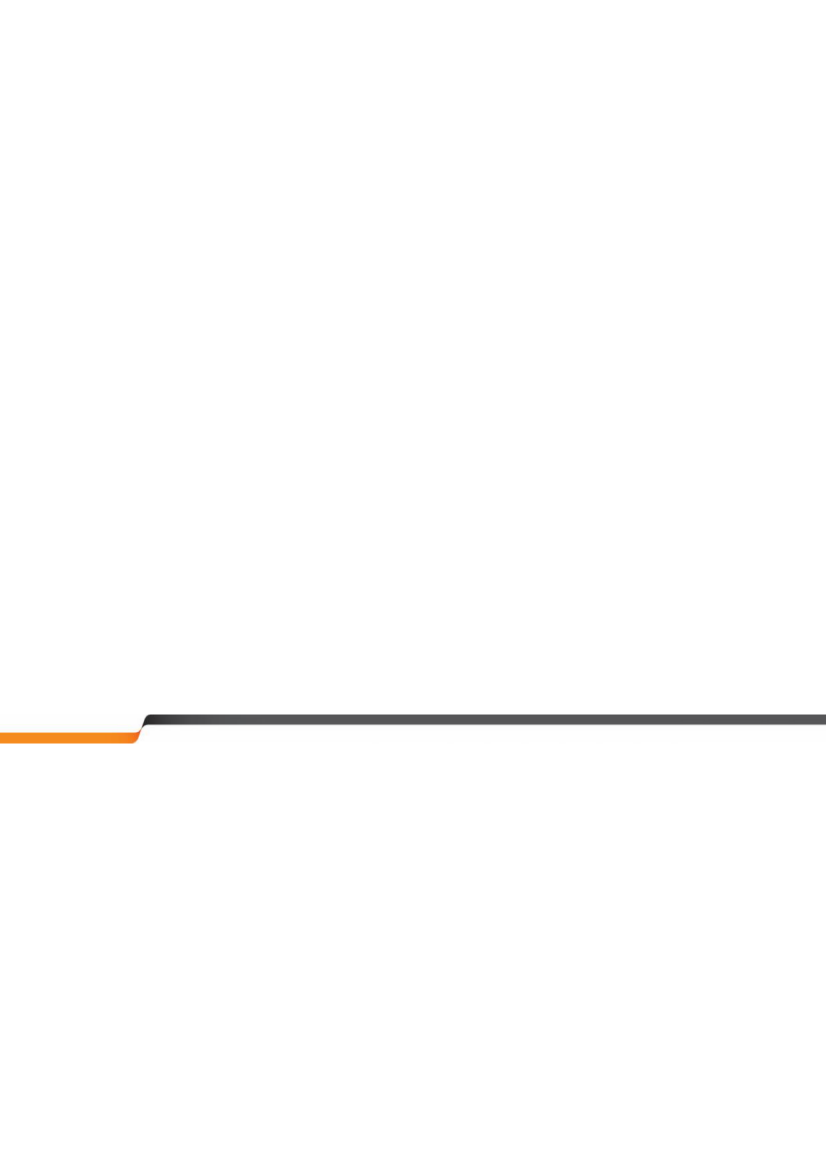
\includegraphics[width=\paperwidth,height=\paperheight,%
keepaspectratio]{viiva}%
\vfill
}}}


\makeatletter
\renewcommand{\maketitle}{
\thispagestyle{empty}
\ThisCenterWallPaper{1}{viiva}
%
\vspace*{9.5cm}
\tn{\LARGE \@author\\[0.75cm]\Huge \@title}\\[3.5cm]

\parbox{.7\linewidth}{\normalsize 
Helsinki Metropolia University of Applied Sciences\\[2pt]
\metropoliadegree \\[2pt]
\metropoliadegreeprogramme \\[2pt]
%Thesis\\[2pt]
\ddmmyyyydate\today}%to be checked date format? 

\ThisLRCornerWallPaper{1}{metropolia}
%
\clearpage
}
\makeatother

\makepagestyle{abstract}
\makeevenhead{abstract}{}{}{Abstract}
\makeoddhead{abstract}{}{}{Abstract}

%----------------------------------------------------------------------------------------
%	START OF THE CONTENT
%----------------------------------------------------------------------------------------
\begin{document}
\tracingall
\counterwithout{lstlisting}{chapter}

\newcommand\tn[1]{\textnormal{#1}}
\newcommand\reaction[1]{\begin{equation}\ce{#1}\end{equation}}

%page number always on the top right, clear the "chapter/section" head
\pagestyle{myheadings}
\markright{}
%clear chapter "title" foot page
\makeevenfoot{plain}{}{}{}
\makeoddfoot{plain}{}{}{}

%----------------------------------------------------------------------------------------
%	TITLE PAGE
%----------------------------------------------------------------------------------------

\maketitle
\newpage


%----------------------------------------------------------------------------------------
%	ABSTRACT
%----------------------------------------------------------------------------------------

\pagestyle{abstract}
\ThisLRCornerWallPaper{1}{footer}

\begin{tabular}{ | p{4,7cm} | p{10,3cm} |}
  \hline
  Author(s) \newline
  Title \newline\newline 
  Number of Pages \newline
  Date
  & 
  \makeatletter
  \@author \newline
  \@title \newline\newline
  \pageref{LastPage} pages + \total{chapter} appendices \newline %! if no appendices, risk to count total of chapter :D
  \@date
  \makeatother
  \\ \hline
  Degree & \metropoliadegree
  \\ \hline
  Degree Programme & \metropoliadegreeprogramme
  \\ \hline
  Specialization option & \metropoliaspecialisation
  \\ \hline
  Instructor(s) & \metropoliainstructors
  \\ \hline
  \multicolumn{2}{|p{15cm}|}{
  	Project's main objective was to develop an embedded software for Zumo robot control. To achieve this goal elementary theorems had been learned. These basics include but not restricted to numerical representation in 2's complement format, boolean algebra, PWM modulation and PID control. Study of technical manual and electronics datasheets had been necessary.
  	After sufficient knowledge in embedded system programming achieved, the implementation work started with power management to avoid battery ruining.
  	In the next step a basic decision based line following algorithm was developed. The method gave insight how the robot sees the line and how can the current position be measured.
  	To further experiment with the robot control a basic Proportional-Integral-Derivative (PID) control algorithm was developed. Although the code had been finished, it never got fine tuned, only the proportional part is in use with a sufficiently high coefficient. Tests show, by utilizing 4 sensors instead only the two middle, the smoothness of movement can be further increased.
  	Finally a "simple go inside the circle and stay there" algorithm was written for the sumo-style contest.
  } \\[14cm] \hline
  Keywords & \metropoliakeywords
  \\ \hline
\end{tabular}
\clearpage

%----------------------------------------------------------------------------------------
%	Acknowledgement ?
%----------------------------------------------------------------------------------------
%\chapter*{Acknowledgement}
%Thanks to my cats Sirnik and Masya for their continuous support.
%\clearpage

%----------------------------------------------------------------------------------------
%	TABLE OF CONTENTS
%----------------------------------------------------------------------------------------

\makeevenhead{plain}{}{}{}
\makeoddhead{plain}{}{}{}
\pagestyle{empty} %remove page number in toc (if longer than 2 pages)
\ThisLRCornerWallPaper{1}{footer}
\tableofcontents*
\pagestyle{empty} %remove page number in toc (if longer than 1 pages)
\ThisLRCornerWallPaper{1}{footer} %add footer image (if longer than 1 page)
\clearpage
\pagestyle{plain}

%list of figure, tables comes here...


%----------------------------------------------------------------------------------------
%    Lyhenteet / Abbreviation
%----------------------------------------------------------------------------------------

\pagestyle{empty}
\ThisLRCornerWallPaper{1}{footer}
\setlength{\parskip}{1cm}
\chapter*{Abbreviation}
\cftaddtitleline{toc}{chapter}{Abbreviation}{}
\begin{table}[h]
\setlength{\tabcolsep}{8pt}
\renewcommand{\arraystretch}{2}
\begin{tabular}{l p{12cm}}
AC	& Alternating current\\
AD(C)	& Analog to digital (converter)\\
DA(C)	& Digital to analog (converter)\\
DC	& Direct current\\
IDE	& Integrated Development Environment\\
IR	& Infrared\\
NiMH	& Nickel-metal hydride\\
PID & Proportional, Integral, Derivate (control)\\
PSoC	& Programmable System on Chip\\
PV	& Process variable\\
PWM & Pulse-width modulation\\
SP	& Set-point\\
UART	& Universal asynchronous receiver-transmitter\\
USB	& Universal Serial Bus\\

\end{tabular}
\end{table}

\newpage

%page number always on top right; also for chapter "title" page
\pagestyle{plain}
\makeevenhead{plain}{}{}{\thepage}
\makeoddhead{plain}{}{}{\thepage}

\setcounter{page}{1} %page 1 should be Introduction

%----------------------------------------------------------------------------------------
%	CONTENT
%----------------------------------------------------------------------------------------
\chapter{Introduction}
The aim of this project was to study existing technologies and possibly discover new methods to effectively control electronic and robotic systems. The fundamentals of embedded system development was examined and an experimental control software was developed. The main objectives of the embedded software was hardware resource management, overall behavior implementation and predefined task perform. Many basic components of the robot and the micro controller had been explored to achieve these tasks. These modules have been presented in this documentation to provide a complete reference.\\
In the next chapter all the theoretical knowledge explained, which required to understand the basic operation of the robot's electronic. The third chapter presents the software's actual way of operation. The last chapter brings conclusion and show a possible direction for future development.

\chapter{Theoretical background}
First part of this chapter gives insight to theoretical electronic knowledge. The second part presents the electronic modules used in the robot and explains their components' operation.

\section{Pulse Width Modulation}
Pulse Width Modulation (PWM) is a modulation method used to encode information on a carrier signal. PWM is mainly used to empower electronic devices. As the modulated signal alternates between 0 and 1 the device gets an average power instead of continuous output. As a result the devices work in transition between OFF and ON states.\\
\begin{figure}[h]
	\centering
	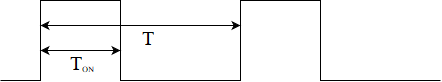
\includegraphics[width=12cm]{illustration/About_PWM}
	\caption[]{PWM cycle}
	\label{fig:aboutpwm}
\end{figure}\\
Duty cycle means the length of ON state (T\textsubscript{on} in figure) during a full cycle (T in figure). The cycle length or frequency can move on wide spectrum from 1 Hz (1 cycle / second) to 10-100 kHz. (See appendix 1, Frequency)\\
In this project 1 cycle is exactly 2.56 ms long as 8 bit timer used. Therefore frequency is approximately 390 Hz. 0 value means no movement, brakes are on during the whole cycle.
\cite{wikipedia:PWM}


\section{PID controller}
Proportional-integral-derivative controller or PID controller is a control loop mechanism. The desired position called setpoint (SP). The measured position referred as process variable (PV). The difference of these values give the error value $ e(t) $. Based on this error value a new corrected position calculated. Calculation formula has 3 main parts each influencing differently the output.\\
\begin{figure}[h]
	\centering
	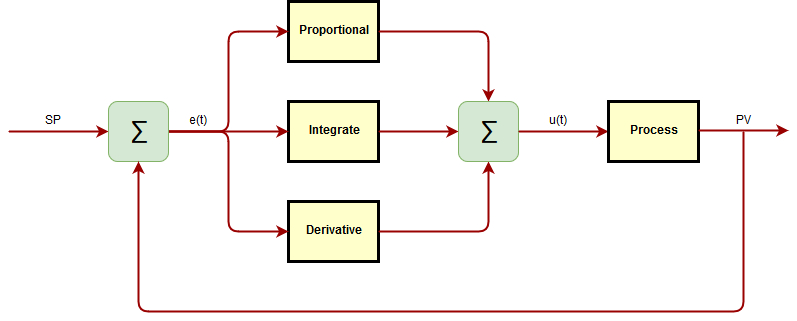
\includegraphics[width=12cm]{illustration/PID_controller}
	\caption[]{PID controller diagram}
	\label{fig:pidcontroller}
\end{figure}\\
The proportional part is contributing linearly, greater current $ e(t) $ error value results in greater correction.
The integral part collects and integrates past error values. When this integrated error applied, it replaces the error deviation caused by proportional correction. As a result the quickly changing proportional correction replaced by a slowly changing integral correction and the function gets dampened.
The derivative part gives a future estimate based on the current changes in the function. It try to zero out the error change rate. Hence the derivative part cannot bring the error to zero.\\
\begin{align}
u(t) = K_{p}e(t) + K_{i} \int_{0}^{t} e(\tau)d\tau + K_{d} \dfrac{de(t)}{dt}
\end{align}\\
This mathematical formula contains all three parts. If any part is not to be applied the respective coefficient values should be set to 0. Usually the integral, the derivative or both.
\cite{wikipedia:PID}
\cite{Lectures}

\section{Cypress CY8 modeling kit}
Cypress CY8CKIT is an Arm Cortex M3 based inexpensive prototyping kit. It includes a programmer and debugger modul, making development easier. It is programmed through USB connection. Output terminal is provided on UART port emulated over the USB connection. Software development and device firmware writing performed with PSoC Creator IDE software provided by Cypress, the kits manufacturer.\cite{cy8ckit}

\section{Zumo robot}
The Pololu Zumo is a small size (less than 10cm) tracked base robot platform. The motors and controller are replaceable allowing customized builds. It includes a steel plate, mounted at the front to protect electronics and to provide capability to push objects. Power source is 4 pieces of AA battery.\cite{zumo}

\subsection{Power management}
The Zumo robot is powered by 4x 1,2V NiMH batteries. The micro controller runs with 5V and 0V. In order to protect the batteries form too low discharge the voltage is constantly measured. If the voltage drop low the user has to be notified using the led light on the robot.\\
Because the micro controller operates with clean 5V, and the fully charged batteries reach up to 1.4V each (sum up in 5.6V) the actual voltage is scaled down to 2/3 (See appendix 1, Voltage division rule). This lowered voltage is then directed to micro controllers AD converter unit.\cite{Lectures}

\subsection{Motor control}
Zumo's motors are 6V DC motors.
\begin{itemize}
	\item Idling: no acceleration and minimum force. Power input: 120mA at 6V.
	\item Stall: 1.6A / motor. Motor controller restricts current to 1.5A / motor.
	\item Speed: Run at 400 RPM. The installed gearbox's ratio is 75:1. The top speed is approximately 60 cm/s.
\end{itemize}
Motor controller unit connects batteries to both motors as instructed by control signals. Motor controller contains H-bridges (DRV 8835). DRV 8835 contains 2 bridges, thus capable to control 2 motors simultaneously.\\
\begin{figure}[h]
	\centering
	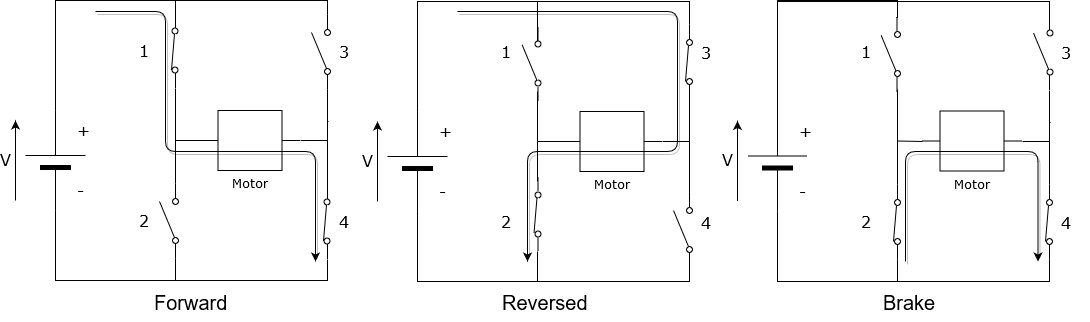
\includegraphics[width=15cm]{illustration/H-bridge}
	\caption{3 states of motor controller}
	\label{fig:h-bridge}
\end{figure}\\
Electronically there are 3 states the H-bridge can be.
\begin{itemize}
	\item Forward: direction set to 0, PWM set to 1
	\item Reverse: direction set to 1, PWM set to 1
	\item Brake: direction left as it was before braking, PWM set to 0
\end{itemize}
In brake mode the motor has changed to generator and shorted. In practice this means wheels locked. There is no mode when wheels can freely roll.
\cite{Lectures}

\subsection{Line detection sensors}
Zumo has 6 infrared light based sensor positioned at the front. Because IR light is out of visible spectrum, 2 red light led also placed on board. The IR led's light reflected from the surface under the robot back to the sensors. Amount of reflected light is measured using indirect AD conversion. Reflected light activates IR sensitive transistor which close circuit. The current flowing in the circuit is integrated in a capacitor until voltage reach defined level. Time to reach defined level is measured with a micro controller counter. If the surface is white, it has good reflection, so the big current charge the capacitor in short time.\\
The actual measurement happens in three steps.
\begin{itemize}
	\item Initial situation: Even when no measurement is happening some current might still flow eventually charging up the capacitor.
	\item Capacitor discharge: When the micro controller measurement pin gives 5V output, on both sides of the capacitor will be 5V. Consequently the capacitor discharge in 1\ldots2 \textmu s.
	\item Measurement: Micro controller measurement pin set to input and a timer is started. Capacitor starts to charge again as fast as the IR-sensitive transistor allows it. When capacitor charge reach about 2.5V, voltage at measurement point drops below 2.5V and the pin value turn to 0. Capacitor keeps charging up to 5V. Time to turn from 1 to 0 is measured.
\end{itemize}
Measurement procedure always takes 1 ms. Different sensors have different sensitivities. Environmental lighting also affects measurement as sun light contains plenty of infrared light.\cite{Lectures}

\chapter{Realization}
In this chapter the process of project development is presented including code explanation and the circumstances of experimenting with Zumo robot.

\section{The embedded software and mechanics}
The section explains algorithms as they control different parts of the robot, introduced in the previous chapter. Movement controlling formulas and program flows also explained.

\subsection{Voltage measurement}
\begin{sloppypar}
Library for battery management is named \textless ADC\_Battery\textgreater . It is part of micro controller standard library and the source can be found in 'codegentemp' folder. Prior to use, it has to be initialized with ADC\_Battery\_Start() command.
Actual measuring is not instantaneous. The process is started with the ADC\_Battery\_StartConvert() command.\\
Wait to finish measurement is achieved in one step: ADC\_Battery\_IsEndConversion(ADC\_Battery\_WAIT\_FOR\_RESULT).
The actual value is queried with ADC\_Battery\_GetResult16() instruction. As the micro controller operates with 5V, measurement range is 0V - 5V. The AD converter is 12 bits unsigned therefore the return value is in 0 - 4095 interval. The formula of actual voltage:
\end{sloppypar}
\begin{align}
volts = \dfrac{AD code}{4095} * 5 * 1.5
\end{align}
. As mentioned in Chapter 2's Zumo robot section, battery voltage scaled down to 2/3. The trailing multiplication by 1.5 in the formula compensates this scale down.

\subsection{Decision based line following}
Decision based line following algorithm is recommended to develop first. It is straightforward to implement and it can provide insight how the sensors see the path. Also help understand the characteristic and dynamic of the motors, how the small changes affect the robot's overall movement.\\
This method use two state, black and white values only. If the threshold parameters set accurately the method can operate in various light conditions.
\begin{figure}[h]
	\centering
	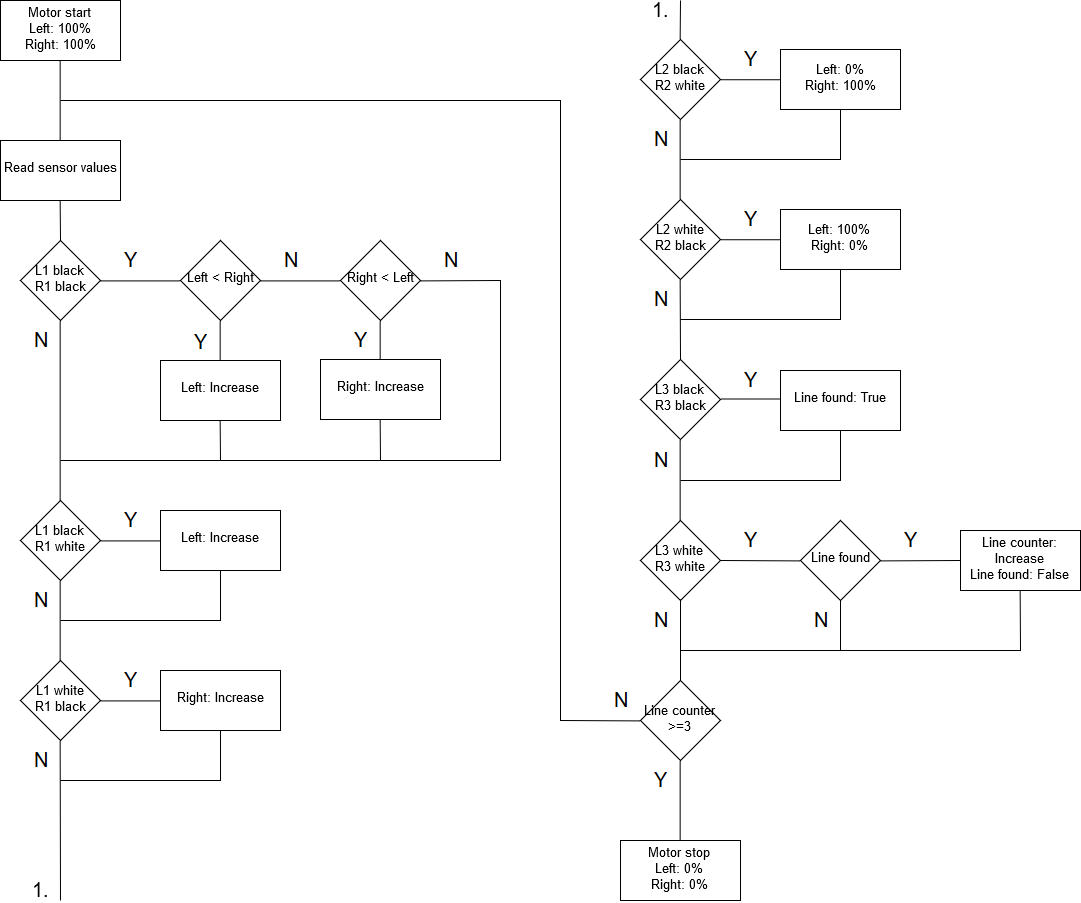
\includegraphics[width=15cm]{illustration/If-then-algorithm}
	\caption{Line following mechanism}
	\label{fig:If-then-algorithm}
\end{figure}\\
This algorithm utilizes all 6 sensors to navigate along the path. The middle two sensors used in two ways. If both read black value, the robot motor speeds are increased toward equal values, thus bringing the robot to straight. If one sensor measure black but the other one white, it is regarded as small deviation from path and minor speed adjustment applied. The two mid-end sensors detect greater deviation from path and utilize larger corrections. The two end sensors used for path intersection detection only.\\
Crossing lines detected in two step by recognizing black-to-white transitions.
\begin{itemize}
	\item In first step, if both sensors report black value, Line\_found flag is set.
	\item Secondly, if sensors read white values and Line\_found flag is 1 means the robot just passed from black to white. Consequently line counter variable increased and the flag set to 0.
\end{itemize}
Experiments has shown, if-then control can be used to 'convert' smooth path to polygonal track. If the curvatures regarded as rough polygons, the robot movement becomes straight run with sudden direction changes resulting in faster method, than what PID control can provide.

\subsection{PID control and error calculation}
This method can provide the most accurate line following. It results in smooth although not the fastest run.\\
First an error rate must be calculated. It is based on the two middle sensor's average value.
\begin{align}
ErrorRate = \dfrac{BlackValue - AverageReading}{BlackValue - WhiteValue}
\end{align}
The error rate should be between 0 and 1. Because $BlackValue$ and $WhiteValue$ contains some tolerance (to cover lighting circumstances), error rate can be outside of these boundaries. The direction of deviation also included in the value. Negative sign means deviation to the left side, positive means to the right.\\
Next the integral and derivative parts are calculated.
\begin{align}
Integral = Integral + ErrorRate * DeltaTime
\end{align}
\begin{align}
Derivative = \dfrac{Error - PreviousError}{DeltaTime}
\end{align}
In following step, the $ErrorRate$, $Integral$ and $Derivative$ values are multiplied by their respective coefficients and summed up. The absolute value of result is calculated. Finally, based on the sign of error rate (indicates direction) correction is applied to opposite side motor speed. (If robot is on left side of track the right motor must brake.)

\subsection{Sharp turn calculation}
If $ErrorRate$ drops to zero, it means the robot lost track completely. In this situation it should find the way back to the path. To achieve this the two end sensor values are continuously monitored. If any of them reads $BlackValue$, the time is recorded. When the track is lost, sharpturn mode turned on. In sharpturn mode PID control is disabled and more direct control utilized.
\begin{figure}[h]
	\centering
	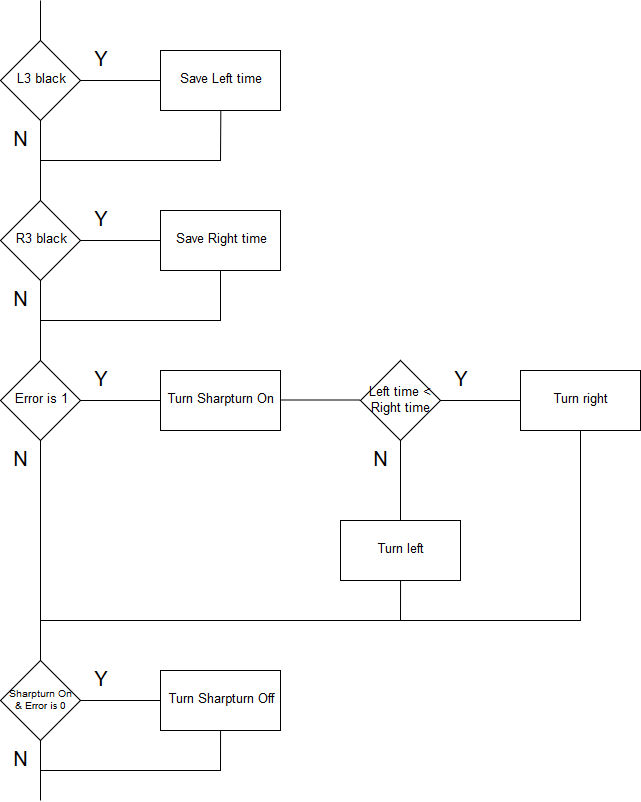
\includegraphics[width=9cm]{illustration/Sharpturn}
	\caption{The sharp turning mechanism}
	\label{fig:Sharpturn}
\end{figure}\\
The robot can not leave the track without reading on any side $BlackValue$, therefore one of the time stamps is indicating where should the robot look for the path.\\
When sharpturn mode is active, the robot motors are programmed with maximal speed, but opposite directions. This way the robot start spinning around its center axis. When $ErrorRate$ becomes again 1 sharpturn mode turned off and control is returned for PID controller.

\subsection{Motor speed programming}
Desired speed value is stored in percentage. 100\% means the preset travel speed value. It is also signed value. Positive sign means forward, while negative sign means reversed direction movement.\\
\begin{align}
ActualSpeed = \dfrac{DesiredSpeed * TravelSpeed}{100}
\end{align}
After the calculations of left and right side speeds, the absolute values are programmed into the PWM controller.\\
Finally the motor directions programmed according to the sign of desired speed.

\section{Timing}

\begin{figure}[h]
	\centering
	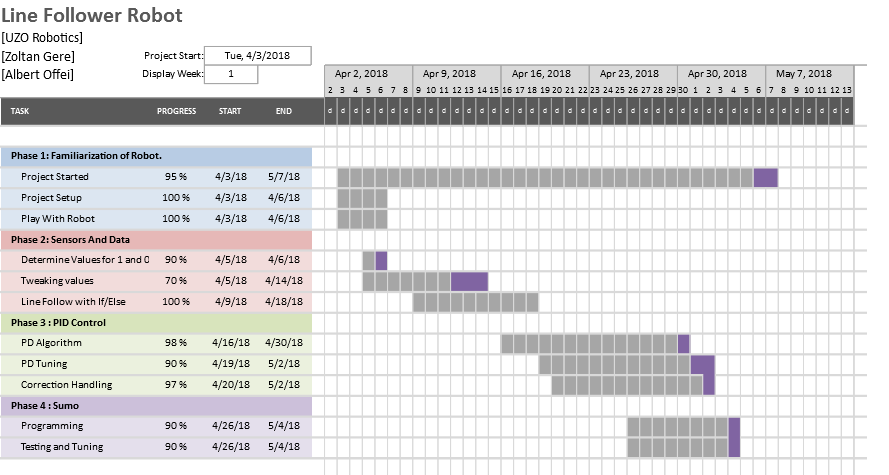
\includegraphics[width=15cm]{illustration/development_timeline}
	\caption{Development timeline}
	\label{fig:dev_timeline}
\end{figure}
The work phases distribution over time is presented here.

\subsection{Familiarisation Of Robot}

\subsection{Project Setup}
PSoC creator software was downloaded and installed. Github was used as version control. To achieve this, one member of the group created a Github repository and other members were added as contributors. Considering the time frame for the project, a library was provided which had the hardware and the various components set up. The code needed to follow the line and to participate in the Sumo fight was then programmed using this library. 

\subsection{Play With Robot}
We experimented with the robot forward movement as a first step. The motor\_forward function provided by the library, handles this. The code snippet bellow shows the motor\_forward function.
\vspace{-22pt}\begin{lstlisting}[language=C,caption={Robot Forward Move},label=move.c] 
void motor_forward(uint8 speed,uint32 delay)
{
    MotorDirLeft_Write(0);      // set LeftMotor forward mode
    MotorDirRight_Write(0);     // set RightMotor forward mode
    PWM_WriteCompare1(speed); 
    PWM_WriteCompare2(speed); 
    CyDelay(delay);
}
\end{lstlisting}\vspace{-22pt}
As shown in code snippet  , the motor\_forward function takes uint8 (unsinged 8bit Integer) value of 100 which represents the speed value as the first parameter and 2000 as the delay.  
\vspace{-22pt}\begin{lstlisting}[language=C,caption={Robot Forward Move},label=move.c] 
motor_forward(100,2000);     // moving forward
motor_turn(200,50,2000);     // turn
motor_turn(50,200,2000);     // turn
motor_backward(100,2000);    // moving backward
\end{lstlisting}\vspace{-22pt}

\subsection{Sensors And Data}
The robot uses six reflective sensors. The values provided by the sensors are higher when on black, around 23000 and about 5000 when on white. 
As the robot nears black, the values increases and vice versa. For the Sumo fight, an ultrasonic sensor was used to measure distance. The ultrasonic sensor served as the eye of the robot to determine the proximity of other robots. Reflectance\_start() function from the library was used to start the sensors.
\vspace{-22pt}\begin{lstlisting}[language=C,caption={Reflectance},label=reflectance.c] 
void reflectance_start()
{
    IR_led_Write(1);
    //sensor_isr_StartEx(sensor_isr_handler);
    Timer_R1_Start();
    Timer_R2_Start();
    Timer_R3_Start();
    Timer_L3_Start();
    Timer_L2_Start();
    Timer_L1_Start();
    refl_init = true;
    Systick_Start();
}
\end{lstlisting}\vspace{-22pt}

\subsection{Tweaking Values}
\vspace{-22pt}\begin{lstlisting}[language=C,caption={Reflectance Threshold},label=refthres.c] 
reflectance_set_threshold(9000, 9000, 11000, 11000, 9000, 9000); // set center sensor threshold to 11000 and others to 9000
\end{lstlisting}\vspace{-22pt}
The reflectance\_set\_threshold() function above takes six parameters which are the threshold above which a sensor output is considered a logic 1 and bellow a logic 0. During this phase of the project, we played with several possible values. To do this, we had the robot connected to the laptop without motor running and moved the robot on the black and white to see how the values changed.\\
\begin{figure}[h]
	\centering
	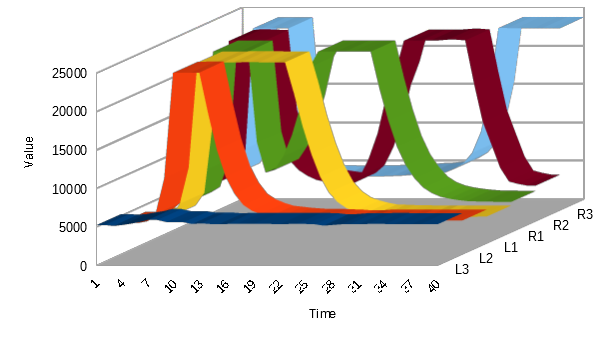
\includegraphics[width=12cm]{illustration/reading_chart}
	\caption[Value set read by the sensors]{Value set read by the sensors}
	\label{fig:readingchart}
\end{figure}
As the robot had been moved over the black line we get the above sensor values. The peak values form the black line and the low 'valley' values represent the white background.

\subsection{Line Follow With If/Else}
\vspace{-22pt}\begin{lstlisting}[language=C,caption={If/Else Line Follow},label=follow.c] 
 //IF AND ELSE STATEMENTS WITH DIGITAL VALUES OF 4 MIDDLE SENSORS
       
    if (!dig.l2 &&dig.l1 && dig.r1 && !dig.r2) // (0110)all clear condition
    {
        motor_forward(255, 10);
    }
    
    else if (dig.l2 && dig.l1 && !dig.r1 && !dig.r2) // (1100)smaller turn here to the left
    {
         motor_turn(0,180,10);
    }
    
    else if (dig.l2  && !dig.l1 && !dig.r1 && !dig.r2 ) //(1000) faster turn to the left
    {
       // motor_turn(0,180,10);
         MotorDirRight_Write(0);
        MotorDirLeft_Write(1);
        if (dig.l1 && dig.r1)
        {
            MotorDirRight_Write(0);
            MotorDirLeft_Write(0);
            motor_forward(255,10);
        }
        
    }
    
    else if (!dig.l2 && !dig.l1 && dig.r1 && dig.r2) // (0011)smaller turn here to the right
    {
        
        motor_turn(180,0,10);
        
    }
    
    else if (!dig.l2  && !dig.l1 && !dig.r1 && dig.r2 ) //(0001) faster turn to the right
    {
       
        MotorDirRight_Write(1);
        MotorDirLeft_Write(0);
        if (dig.l1 && dig.r1)
        {
            MotorDirRight_Write(0);
            MotorDirLeft_Write(0);
            motor_forward(255,10);
        }
    } 
\end{lstlisting}\vspace{-22pt}
Using the above code, the robot was able to follow the line considerably well albeit not smoothly enough. The If/Else code above, takes into account the digital values that the sensors output which was determined during our value tweaking phase. From the first If statement, the motor\_forward function takes the maximum speed value of 255 and a delay of 10 milliseconds, if both middle sensors are on black and hence has a value of 1. After 10 milliseconds, the condition is checked again and moves to the next code if condition has changed. 
The first else if condition statement, checks if sensor l2 and l1  can both see black and if r2 and r1 both see white, in that case, we give the left motor a speed of 0 and the right motor a speed of 180 cause the robot to turn left. A  check was performed again after 10milliseconds. This approach worked for simple turns but failed at sharper turns. 
We found that one way to work the sharper turns was to make use of the motor\_backwards function of the library.  
\vspace{-22pt}\begin{lstlisting}[language=C,caption={motor\_turn and motor\_backwards},label=backwards.c]
void motor_turn(uint8 l_speed, uint8 r_speed, uint32 delay)
{
    PWM_WriteCompare1(l_speed); 
    PWM_WriteCompare2(r_speed); 
    CyDelay(delay);
}


/**
* @brief    Moving motors backward
* @details  setting backward mode to each motors and gives same speed to each side of PWM
* @param    uint8 speed : speed value
* @param    uint32 delay : delay time
*/
void motor_backward(uint8 speed,uint32 delay)
{
    MotorDirLeft_Write(1);      // set LeftMotor backward mode
    MotorDirRight_Write(1);     // set RightMotor backward mode
    PWM_WriteCompare1(speed); 
    PWM_WriteCompare2(speed); 
    CyDelay(delay);
}
\end{lstlisting}\vspace{-22pt}

\chapter{Conclusion}
The objective of this project was to develop controlling software for Zumo robot. It has been accomplished, as the robot is capable of following the path up to the finish line. During development and race the robot worked well and batteries have been spared.\\
The if-then method works well. The PID controller also works on algorithm level. It can not be used yet, as fine tuning of parameters is necessary. But if the robot is intended for racing, the if-then approach should be further developed and tuned, because PID controller gives smoother but slower result.\\
Development might be considered successful on educational level. Developers acquired basic electronic, device, programming and controlling knowledge. These can be used in future researches and developments.

%----------------------------------------------------------------------------------------
%   BIBLIOGRAPHY 
%----------------------------------------------------------------------------------------
\newpage
\bibliographystyle{vancouver}
%line space
%\singlespacing %removed otherwise the appendix are also single space
\begin{flushleft}
\begin{singlespacing}
\bibliography{biblio}
\end{singlespacing}
\end{flushleft}

%for conting the pages
\label{LastPage}~


%----------------------------------------------------------------------------------------
%   APPENDICES 
%----------------------------------------------------------------------------------------
%avoid that the last page of bib get appendix header
\clearpage
%start appendix
\appendix
%no page number for appendix in table of content
\addtocontents{toc}{\cftpagenumbersoff{chapter}}
%appendix sections and subsections not in table of content
\settocdepth{chapter}
%add "Appendices" in the table of content
\addappheadtotoc
%force smaller vertical spacing in table of content
%!!! There can be some fun depending if the appendices have (sub)sections or not :D
% You will have to play with these numbers and eventually copy the \pretocmd line on before some \chapter and force another number.
\addtocontents{toc}{\vspace{11pt}}
\pretocmd{\chapter}{\addtocontents{toc}{\protect\vspace{-24pt}}}{}{}

%have Appendix 1 (instead of Appendix A)
\renewcommand{\thechapter}{\arabic{chapter}} 

%each appendix restart page num to one
\setcounter{page}{1}
%special counter for appendix TODO: this is a ugly quick hack :( Should find a better way to count the page per appendix.
\newtotcounter{appx1}
%overwrite the header
\makeevenhead{plain}{}{}{Appendix \thechapter \\ \thepage (\stepcounter{appx1}\total{appx1})}
\makeoddhead{plain}{}{}{Appendix \thechapter \\ \thepage (\stepcounter{appx1}\total{appx1})}

\chapter{Physics}\label{appx:first}
\section{Frequency}
Frequency means for periodical functions (e.g. signals) the number of periods completed in 1 second. Unit of frequency is Hertz (Hz). For example 1 period in 1 second is 1 Hz. 10 period in 1 second is 10 Hz.

\section{Infrared light}
Infrared light (IR) is 700nm to 1mm section of light spectrum. The wavelength of IR is longer than that visible by human eye. This invisibility gives IR light wide range of purpose.

\section{Electricity}
\subsection{Voltage division rule}
Voltage division is a method to produce output voltage, which is fraction of the input voltage. If 2 resistor connected in series, the input voltage is distributed between them. The output voltage can taken from between the resistors.
\begin{align}
V_out = \dfrac{R_2}{R_1 + R_2} * V_in
\end{align}

\begin{figure}
	\centering
	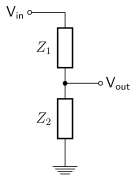
\includegraphics[width=5cm]{illustration/voltage_divider}
	\caption{Voltage divider circuit}
	\label{fig:Voltagedivider}
\end{figure}



%\clearpage % avoid that the last page of previous appendix get this header
%\setcounter{page}{1} %restet to page 1 (you can't avoid this one (I think))
%\newtotcounter{appx2} % to have the total for this appendix and not the previous one.
%overwrite the header
%\makeevenhead{plain}{}{}{Appendix \thechapter \\ \thepage (\stepcounter{appx2}\total{appx2})}
%\makeoddhead{plain}{}{}{Appendix \thechapter \\ \thepage (\stepcounter{appx2}\total{appx2})}

%\chapter{Mathematics}\label{appx:second}

%\section{Appendix Section}

%\subsection{With a Subsection}

\end{document}